% \pragmaonce

% adapted from https://www.overleaf.com/learn/latex/Commands
\providecommand{\dissertationelse}[2]{%
% adapted from https://tex.stackexchange.com/a/33577
\ifdefined\DISSERTATION
#1
\else
#2
\fi
}

../../tex/lib/dissertationonly.tex

\begin{figure*}
  \centering
  \dissertationonly{\footnotesize}
  \begin{tabular}{m{0.05\textwidth}@{}|c@{}|c@{\hskip 0.01\textwidth}|m{0.14\textwidth}}
%-------------------------------------------------------------------------------
\hspace{-1ex}Policy&Lower-Resolution Parameterization&Higher-Resolution Parameterization&\makecell[c]{Properties}\\\hline
%-------------------------------------------------------------------------------
    \rotatebox{90}{\textbf{Fixed Resolution}}
  &
    \makecell{
      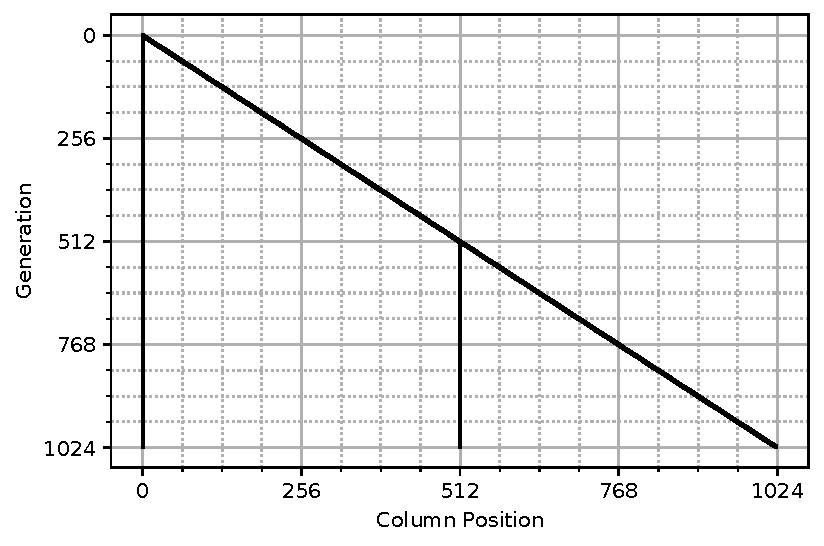
\includegraphics[valign=t,width=\dissertationelse{0.3}{0.4}\textwidth]{submodules/hereditary-stratigraph-concept-binder/binder/retention-policies/teeplots/fixed_resolution=512+num_layers=1024+stratum_retention_predicate=fixed-resolution+viz=tweaked-stratum-retention-drip-plot+ext=}
    }
  &
    \makecell{
      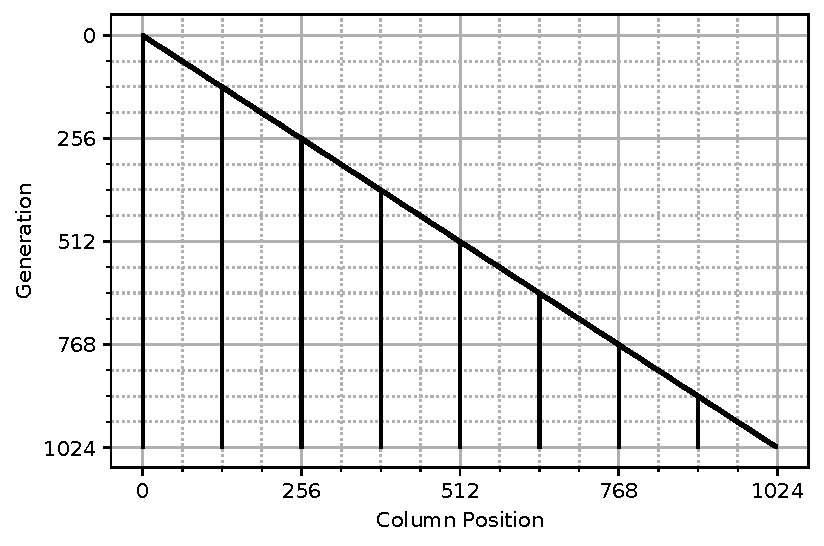
\includegraphics[valign=t,width=\dissertationelse{0.3}{0.4}\textwidth]{submodules/hereditary-stratigraph-concept-binder/binder/retention-policies/teeplots/fixed_resolution=128+num_layers=1024+stratum_retention_predicate=fixed-resolution+viz=tweaked-stratum-retention-drip-plot+ext=}
    }
  &
  \makecell[{{p{0.14\textwidth}}}]{
  \centering
    \bf{Space Complexity}\\
    $O(n)$\\
    \bf{MRCA Uncertainty}\\
    $O(1)$
  }
  \makecell[{{p{0.14\textwidth}}}]{
  \raggedright
    where $n$ is gens elapsed.
  }\\\hline
%-------------------------------------------------------------------------------
    \adjustbox{
      minipage=10em,
      rotate=90,
    }{
      \centering
      \textbf{Depth-Proportional Resolution}
      \par
    }
  &
    \makecell{
      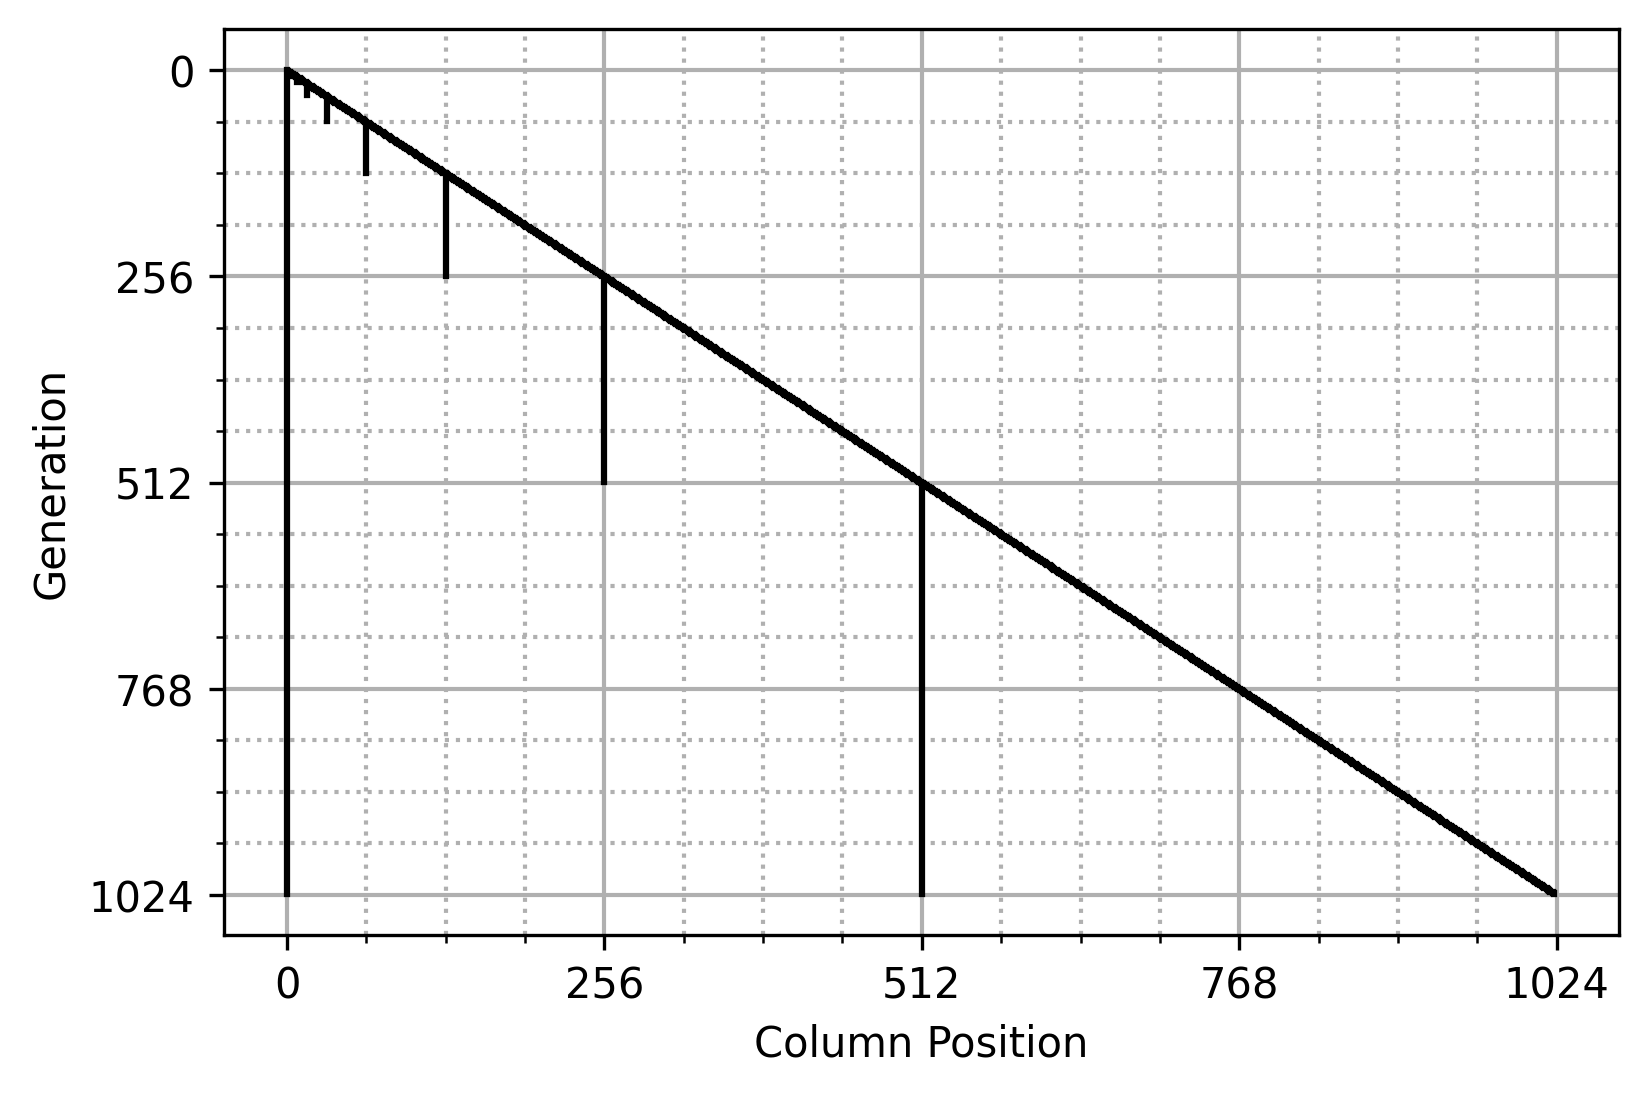
\includegraphics[valign=t,width=\dissertationelse{0.3}{0.4}\textwidth]{submodules/hereditary-stratigraph-concept-binder/binder/retention-policies/teeplots/guaranteed_depth_proportional_resolution=1+num_layers=1024+stratum_retention_predicate=depth-proportional-resolution+viz=tweaked-stratum-retention-drip-plot+ext=}
    }
  &
    \makecell{
      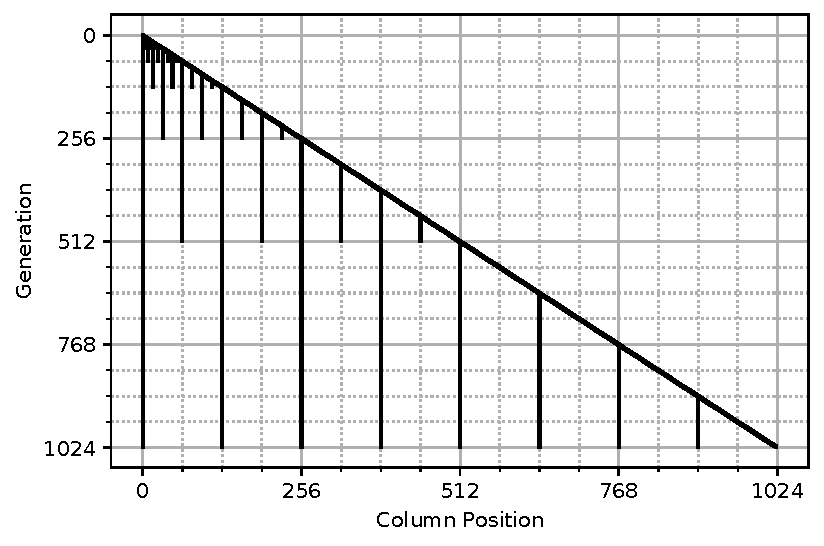
\includegraphics[valign=t,width=\dissertationelse{0.3}{0.4}\textwidth]{submodules/hereditary-stratigraph-concept-binder/binder/retention-policies/teeplots/guaranteed_depth_proportional_resolution=4+num_layers=1024+stratum_retention_predicate=depth-proportional-resolution+viz=tweaked-stratum-retention-drip-plot+ext=}
    }
  &
  \makecell[{{p{0.14\textwidth}}}]{
  \centering
    \bf{Space Complexity}\\
    $O(1)$\\
    \bf{MRCA Uncertainty}\\
    $O(n)$
  }
  \makecell[{{p{0.14\textwidth}}}]{
  \raggedright
    where $n$ is gens elapsed.
  }\\\hline
%-------------------------------------------------------------------------------
    \adjustbox{
      minipage=15em,
      rotate=90,
    }{
      \centering
      \textbf{Tapered Depth-Proportional Resolution}
      \par
    }
  &
    \makecell{
      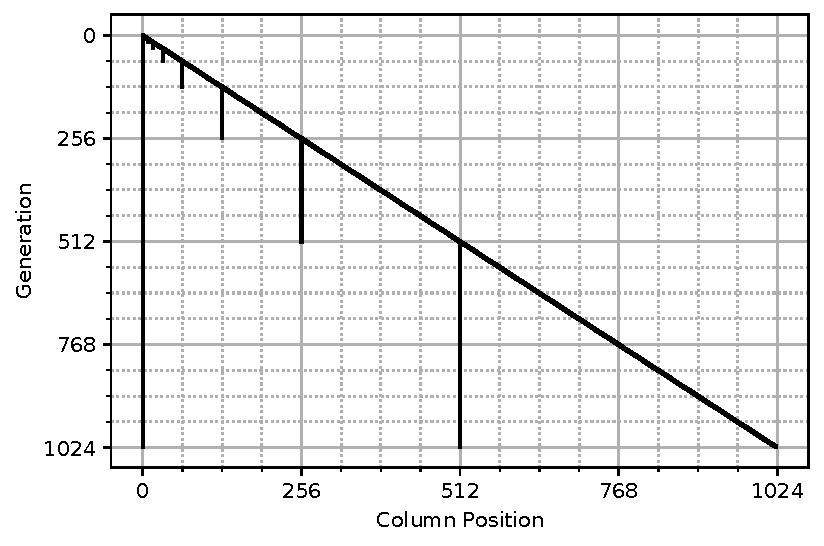
\includegraphics[valign=t,width=\dissertationelse{0.3}{0.4}\textwidth]{submodules/hereditary-stratigraph-concept-binder/binder/retention-policies/teeplots/guaranteed_depth_proportional_resolution=1+num_layers=1024+stratum_retention_predicate=tapered-depth-proportional-resolution+viz=tweaked-stratum-retention-drip-plot+ext=}
    }
  &
    \makecell{
      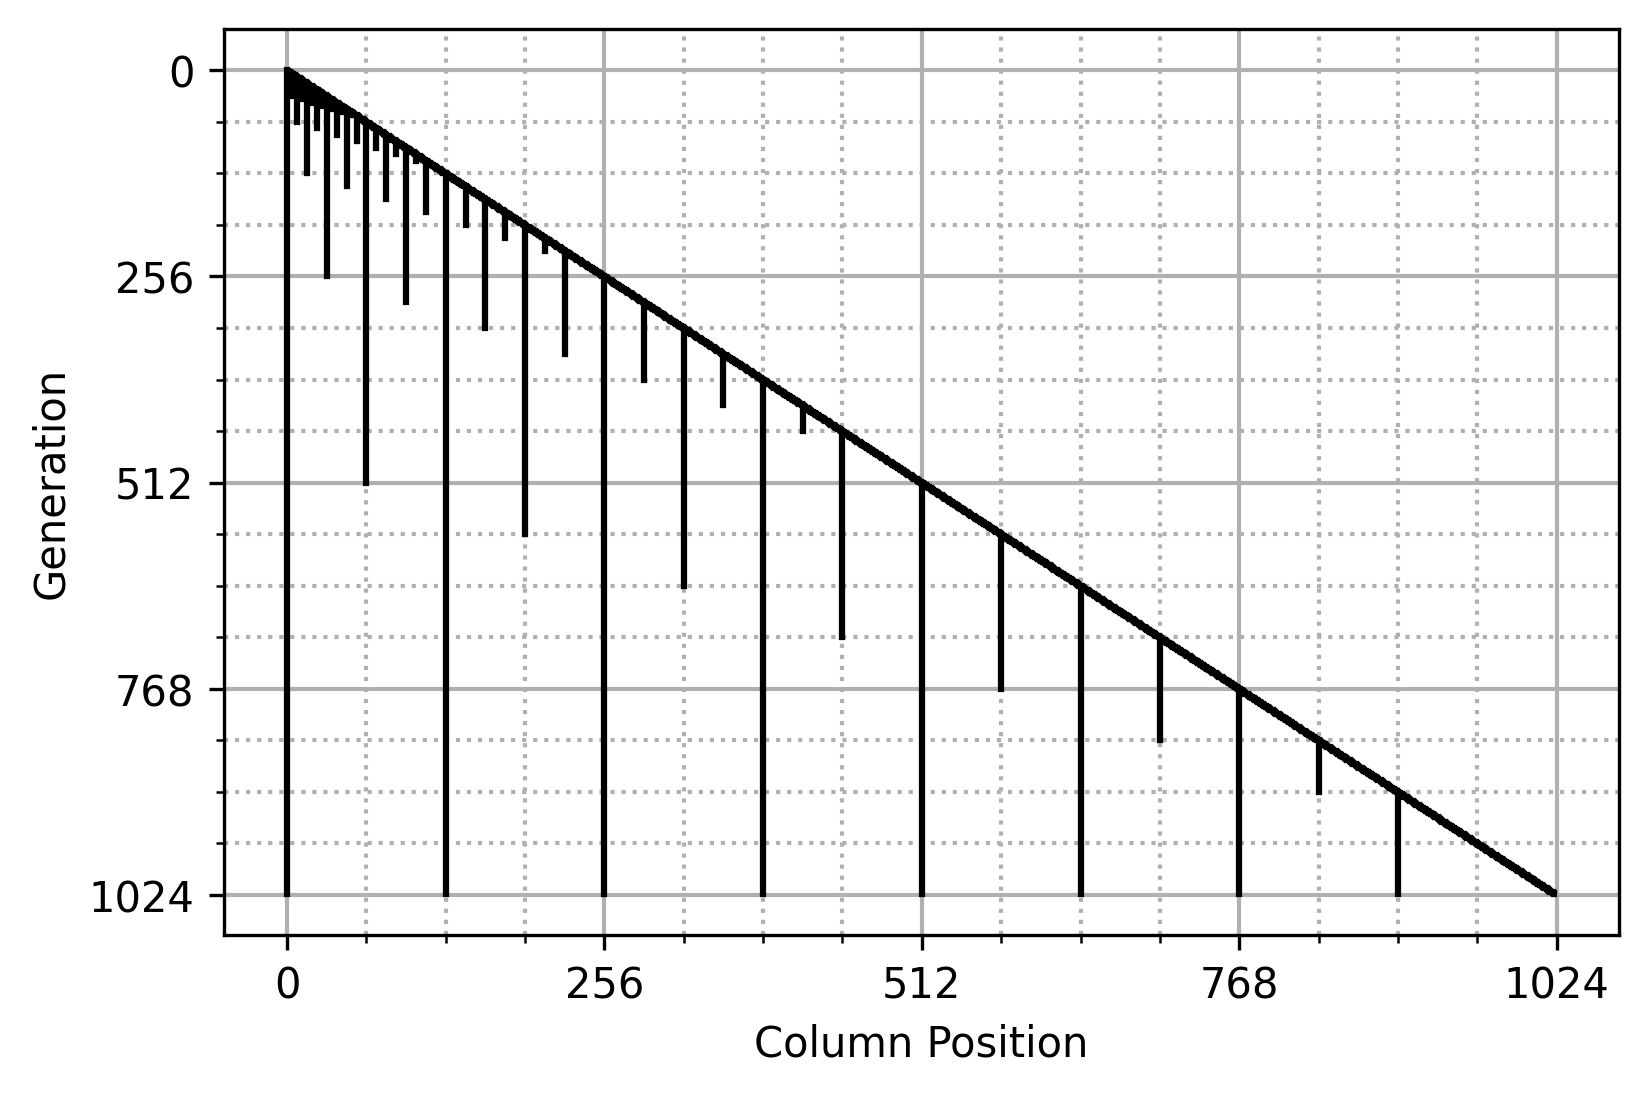
\includegraphics[valign=t,width=\dissertationelse{0.3}{0.4}\textwidth]{submodules/hereditary-stratigraph-concept-binder/binder/retention-policies/teeplots/guaranteed_depth_proportional_resolution=4+num_layers=1024+stratum_retention_predicate=tapered-depth-proportional-resolution+viz=tweaked-stratum-retention-drip-plot+ext=}
    }
  &
  \makecell[{{p{0.14\textwidth}}}]{
  \centering
    \bf{Space Complexity}\\
    $O(1)$\\
    \bf{MRCA Uncertainty}\\
    $O(n)$
  }
  \makecell[{{p{0.14\textwidth}}}]{
  \raggedright
    where $n$ is gens elapsed.
  }\\\hline
%-------------------------------------------------------------------------------
  \adjustbox{
    minipage=15em,
    rotate=90,
  }{
    \centering
    \textbf{Recency-Proportional\\Resolution}
    \par
  }
  &
  \makecell{
    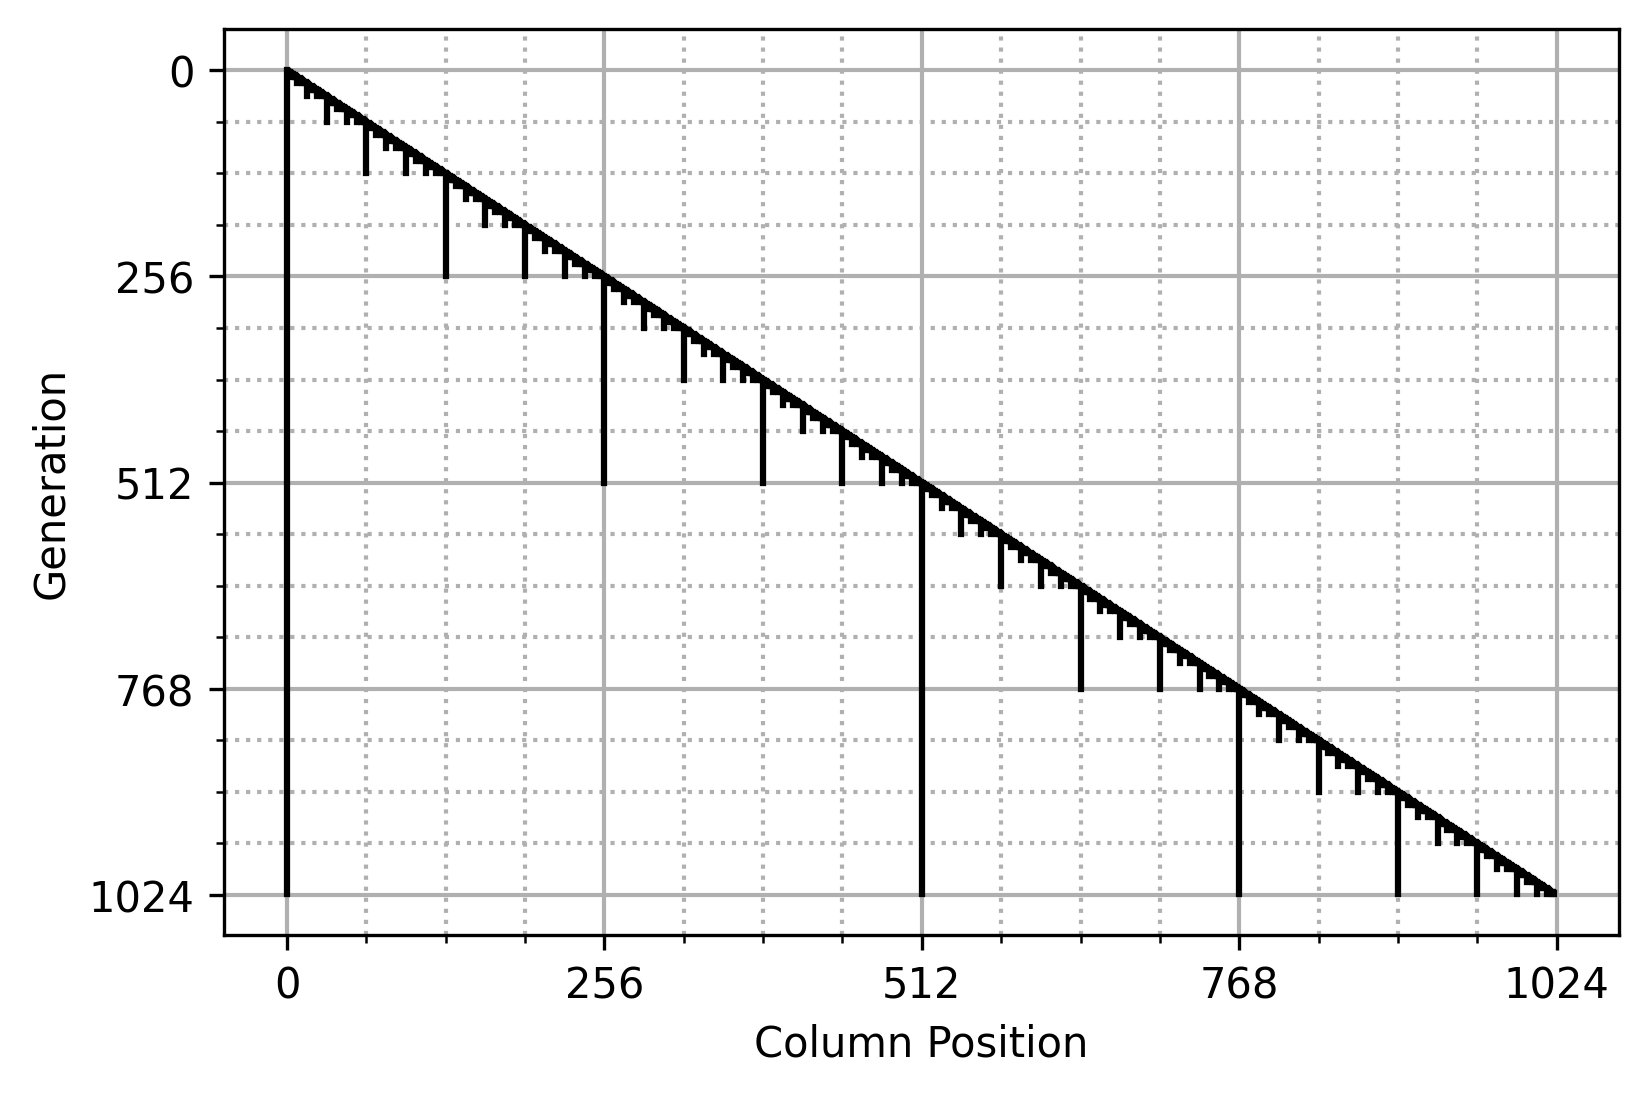
\includegraphics[valign=t,width=\dissertationelse{0.3}{0.4}\textwidth]{submodules/hereditary-stratigraph-concept-binder/binder/retention-policies/teeplots/guaranteed_mrca_recency_proportional_resolution=0+num_layers=1024+stratum_retention_predicate=recency-proportional-resolution+viz=tweaked-stratum-retention-drip-plot+ext=}
  }
  &
  \makecell{
    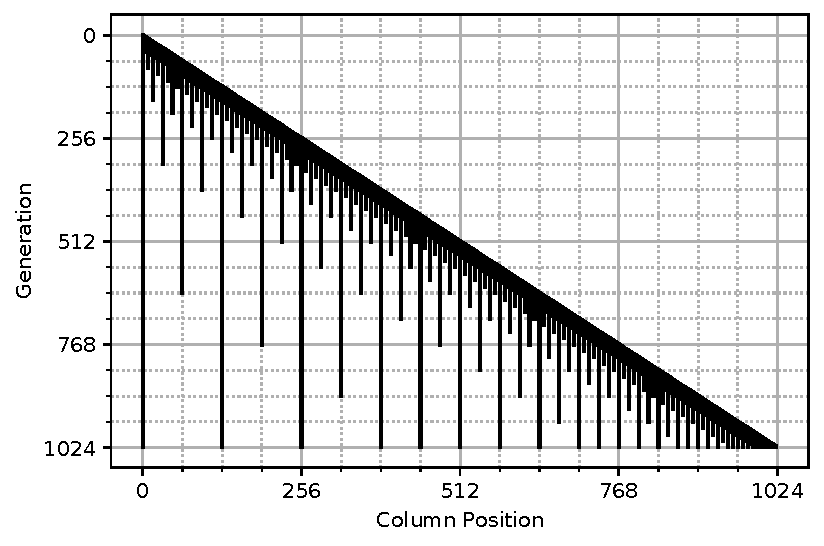
\includegraphics[valign=t,width=\dissertationelse{0.3}{0.4}\textwidth]{submodules/hereditary-stratigraph-concept-binder/binder/retention-policies/teeplots/guaranteed_mrca_recency_proportional_resolution=4+num_layers=1024+stratum_retention_predicate=recency-proportional-resolution+viz=tweaked-stratum-retention-drip-plot+ext=}
  }
  &
  \makecell[{{p{0.14\textwidth}}}]{
  \centering
  \bf{Space Complexity}\\
  $O(\log(n))$\\
  \bf{MRCA Uncertainty}\\
  $O(m)$
  }
  \makecell[{{p{0.14\textwidth}}}]{
  \raggedright
  where $m$ is gens since MRCA and $n$ is total gens elapsed.
  }\\


  \end{tabular}
  \caption{
  Comparison of stratum retention policies.
  Policy visualizations show retained strata in black.
  Time progresses along the $y$-axis from top to bottom.
  New strata are introduced along the diagonal and then ``drip'' downward as a vertical line until eliminated.
  The set of retained strata present within a column at a particular generation $g$ can be read as intersections of retained vertical lines with a horizontal line with intercept $g$.
  Policy visualizations are provided for two parameterizations for each policy: the first where the maximum uncertainty of MRCA generation estimates would be 512 generations and the second where the maximum uncertainty of MRCA generation estimates would be 128 generations.
  }
  \label{fig:retention-policies}
\end{figure*}
